\documentclass[11pt,a4paper]{article}

\usepackage{graphicx}
\graphicspath{{Images/}{./}}

\usepackage[hang,bottom]{footmisc}
\usepackage{adjustbox}
\usepackage{amsmath,amssymb,amsfonts,amsthm}
\usepackage{bm}
\usepackage{natbib}
\usepackage{lipsum}
\usepackage{advdate}
\usepackage{adjustbox}
\usepackage{booktabs} 
\usepackage{tikz}
\usepackage{pdfpages}
\usepackage{caption}
\usepackage{hyperref}
\hypersetup{
    colorlinks=true,
    citecolor=black,
    linkcolor=black,
    filecolor=black,
    urlcolor=black,
    pdfpagemode=FullScreen,
}

\setlength{\textheight}{23.5cm}
\setlength{\topmargin}{-1.05cm}
\setlength{\textwidth}{6.5in}
\setlength{\oddsidemargin}{-0.5cm}

\newtheorem{proposition}{Proposition}
\newtheorem{lemma}{Lemma}
\newtheorem{assumption}{Assumption}
\newtheorem{definition}{Definition}

\begin{document}

\title{Aspirations in the Air:\\ Effect of Development Schemes on AQI}
\author{
Aayushi Agarwal \and
Bhaskar Agarwal \and
Gaurav Banerjee \and
Nandish Patel
}
\date{\today}
\maketitle

\section{Introduction}
Lorem Ipsum

\section{Background}
Lorem Ipsum

\section{Methodology}
Lorem Ipsum

\begin{center}
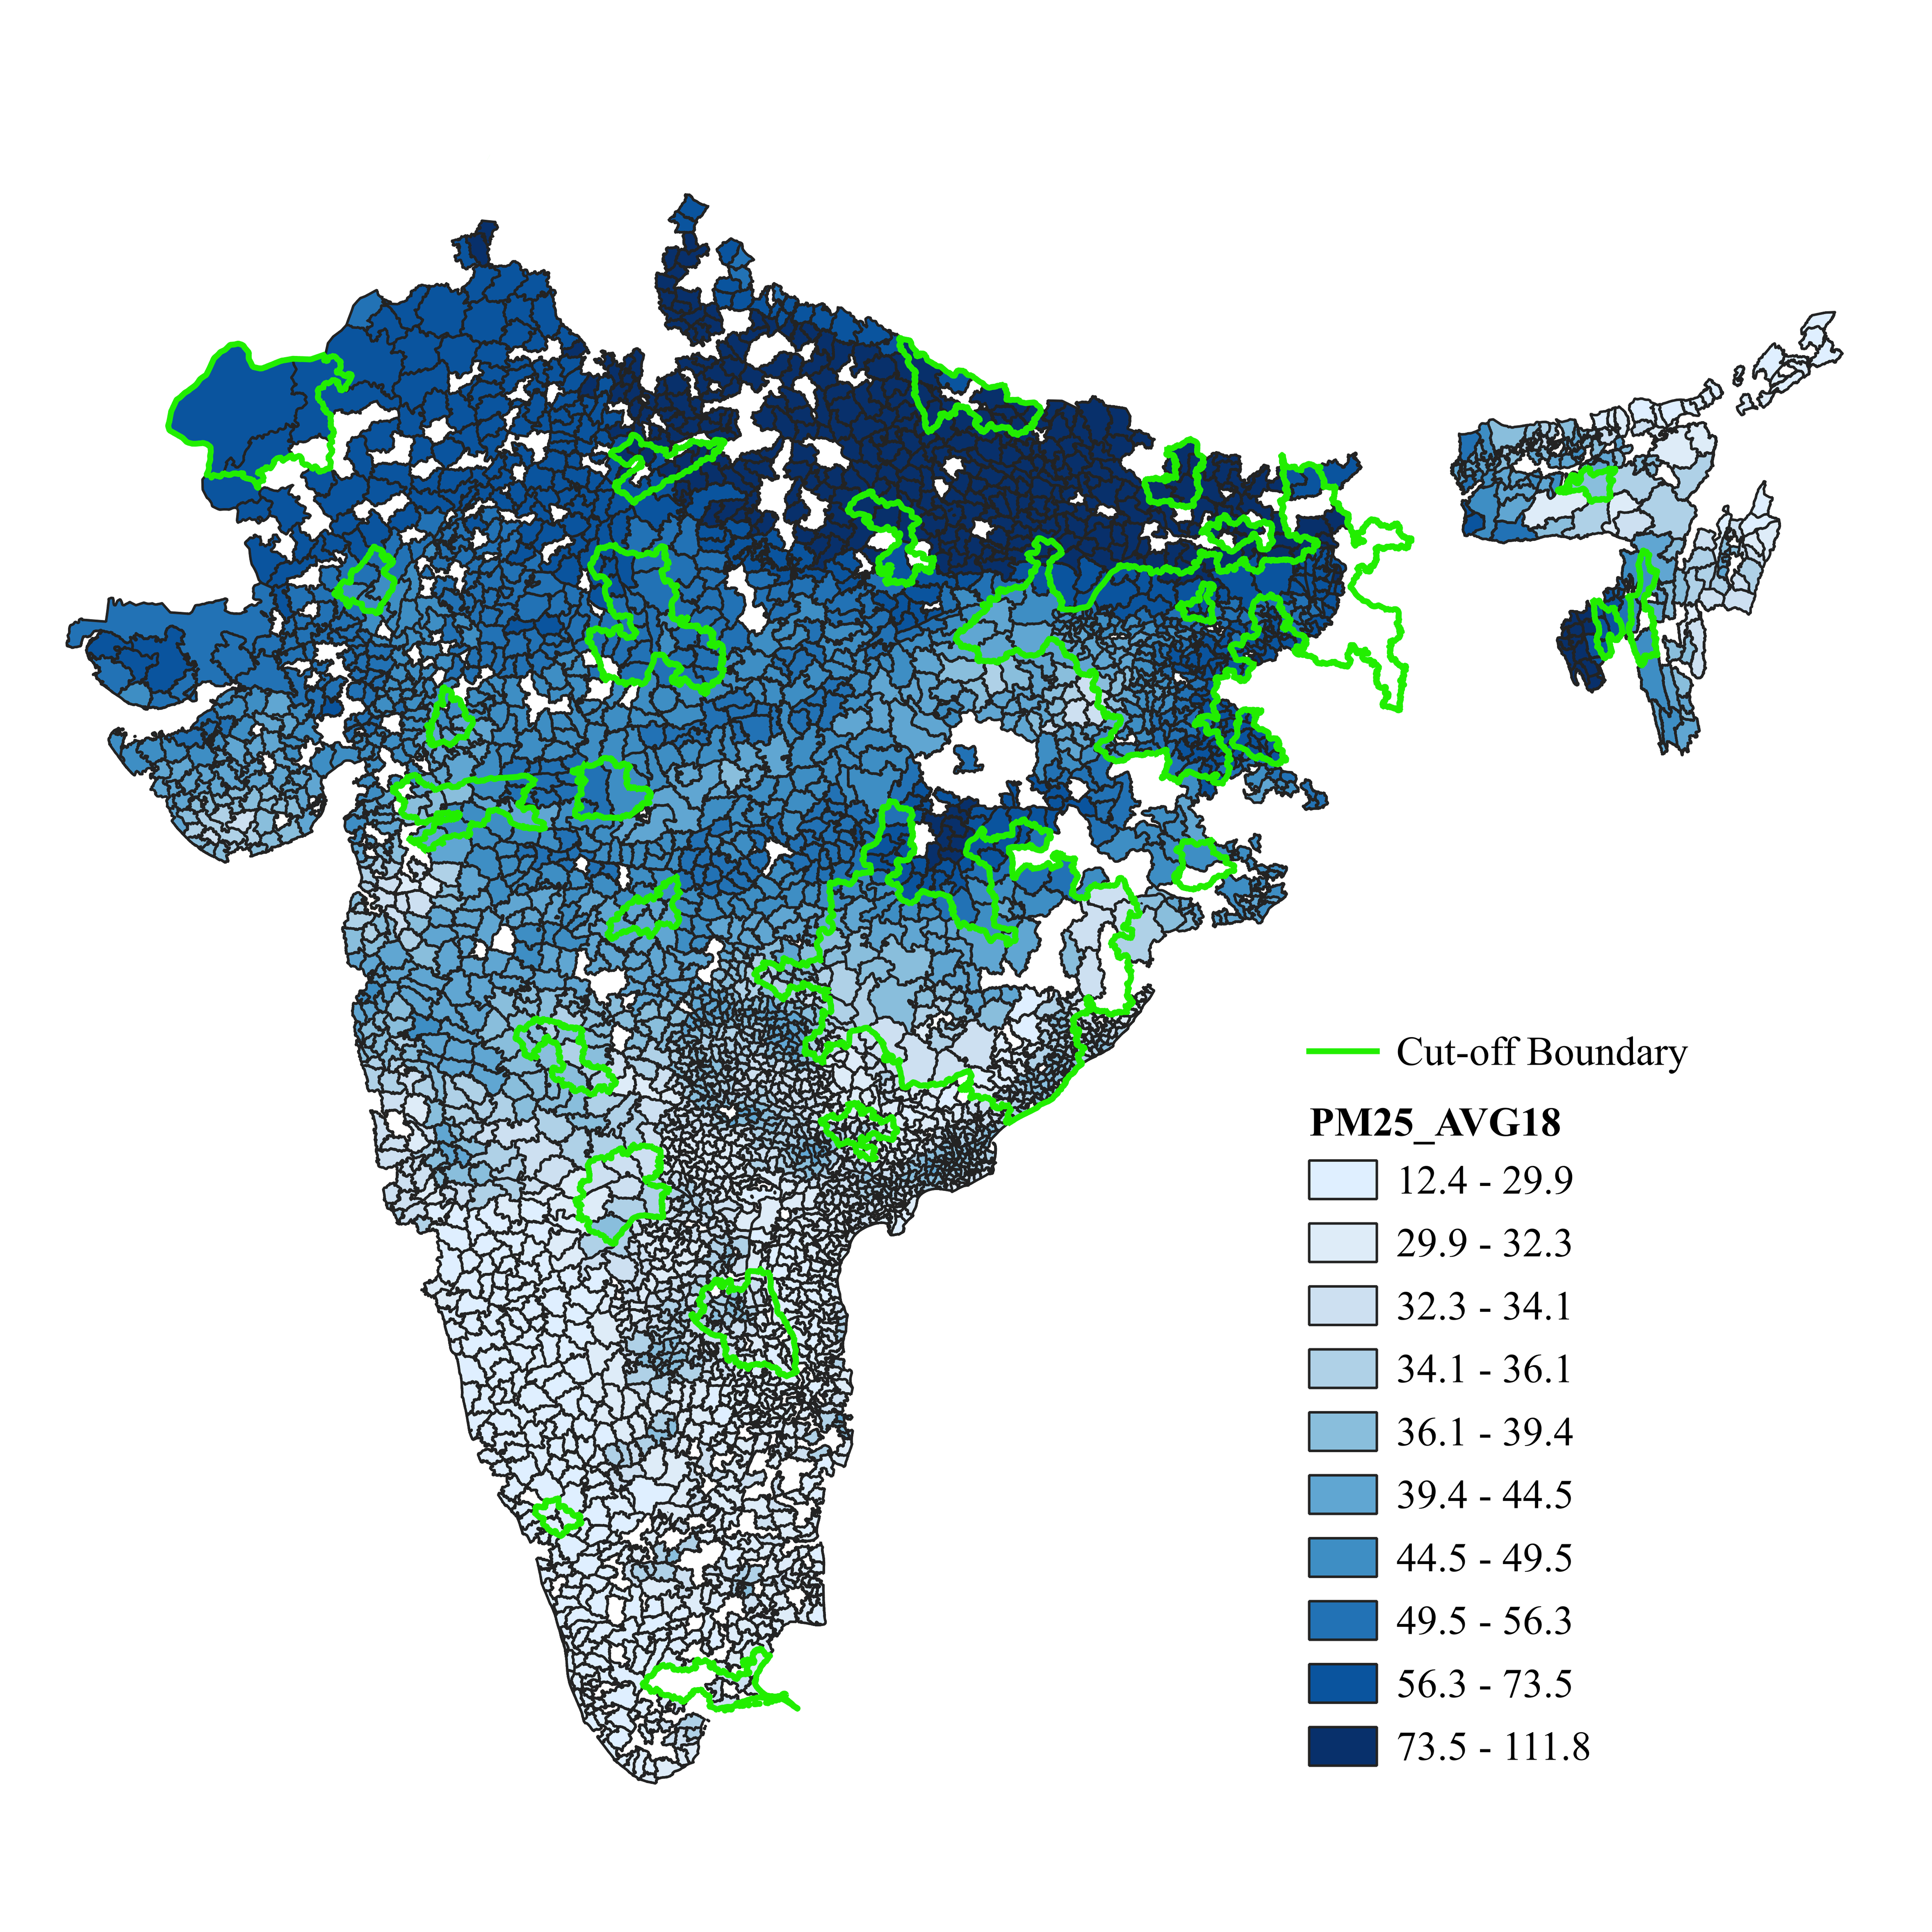
\includegraphics[height=0.25\textheight]{Controls.png}
\end{center}

\section{Empirical Strategy}

\cite{singh1984price}

\section{Results}

\begin{table}[ht] \centering 
  \caption{State-wise Bias-corrected Robust RD Estimates} 
  \caption*{Outcome variable: Mean PM2.5 2018}
\begin{adjustbox}{width=\textwidth}
\begin{tabular}{@{\extracolsep{5pt}} lcccccccc} 
\\[-3.5ex]\hline 
\hline \\[-1.8ex] 
 & Estimate & $95\%$ CI & Std. Error & Robust P-Value & Obs & Eff. Obs & Bandwidth & Covs \\ 
\hline \\[-1.8ex] 
ANDHRA PRADESH & $2.125$ & $[-0.772,5.021]$ & $1.478$ & $0.151$ & $635$ & $116$ & $13.515$ & Yes\\ 
ANDHRA PRADESH & $1.382$ & $[-1.813,4.577]$ & $1.630$ & $0.397$ & $635$ & $128$ & $15.345$ & No\\ 
\hline \\[-1.8ex] 
BIHAR & $14.087$ & $[-128.410,156.585]$ & $72.704$ & $0.846$ & $79$ & $11$ & $7.035$ & Yes\\ 
BIHAR & $-39.645$ & $[-110.808,31.518]$ & $36.308$ & $0.275$ & $79$ & $5$ & $5.643$ & No\\ 
\hline \\[-1.8ex]  
GUJARAT & $3.702$ & $[-14.711,22.115]$ & $9.394$ & $0.694$ & $201$ & $47$ & $36.846$ & Yes\\ 
GUJARAT & $-0.989$ & $[-24.325,22.346]$ & $11.906$ & $0.934$ & $201$ & $47$ & $34.969$ & No\\ 
\hline \\[-1.8ex] 
\textbf{JHARKHAND} & $\textbf{-18.790}$ & $\textbf{[-35.527,-2.054]}$ & $\textbf{8.539}$ & $\textbf{0.028}$ & $\textbf{256}$ & $\textbf{17}$ & $\textbf{4.398}$ & \textbf{Yes}\\ 
JHARKHAND & $ -22.381$ & $ [-40.013,-4.749]$ & $ 8.996$ & $ 0.013$ & $ 256$ & $ 43$ & $ 6.602$ & No\\  
\hline \\[-1.8ex] 
MADHYA PRADESH & $3.868$ & $[-4.513,12.250]$ & $4.277$ & $0.366$ & $259$ & $77$ & $24.041$ & Yes\\ 
MADHYA PRADESH & $6.142$ & $[-2.170,14.454]$ & $4.241$ & $0.148$ & $259$ & $72$ & $21.989$ & No\\ 
\hline \\[-1.8ex] 
MAHARASHTRA & $0.746$ & $[-17.722,19.214]$ & $9.423$ & $0.937$ & $329$ & $53$ & $15.824$ & Yes\\ 
MAHARASHTRA & $-2.357$ & $[-28.844,24.129]$ & $13.514$ & $0.862$ & $329$ & $54$ & $16.327$ & No\\ 
\hline \\[-1.8ex] 
MIZORAM & $8.251$ & $[1.925,14.578]$ & $3.228$ & $0.011$ & $16$ & $15$ & $124.220$ & Yes\\ 
MIZORAM & $23.682$ & $[14.480,32.884]$ & $4.695$ & $0.000$ & $16$ & $15$ & $124.220$ & No\\ 
\hline \\[-1.8ex] 
RAJASTHAN & $29.610$ & $[-25.449,84.670]$ & $28.092$ & $0.292$ & $230$ & $45$ & $17.098$ & Yes\\ 
RAJASTHAN & $31.702$ & $[-26.159,89.562]$ & $29.521$ & $0.283$ & $230$ & $63$ & $25.969$ & No\\ 
\hline \\[-1.8ex] 
TELANGANA & $2.924$ & $[-17.674,23.522]$ & $10.509$ & $0.781$ & $429$ & $23$ & $5.165$ & Yes\\ 
TELANGANA & $-13.303$ & $[-50.241,23.636]$ & $18.847$ & $0.480$ & $429$ & $21$ & $4.833$ & No\\ 
\hline \\[-1.8ex] 
\end{tabular} 
\end{adjustbox}
\caption*{\textit{Notes}. Standard errors are heteroskedasticity robust.}
\end{table} \par

\section{Conclusion}

\bibliographystyle{apalike}
\bibliography{references}

\end{document}
